% This file was created by tikzplotlib v0.9.7.
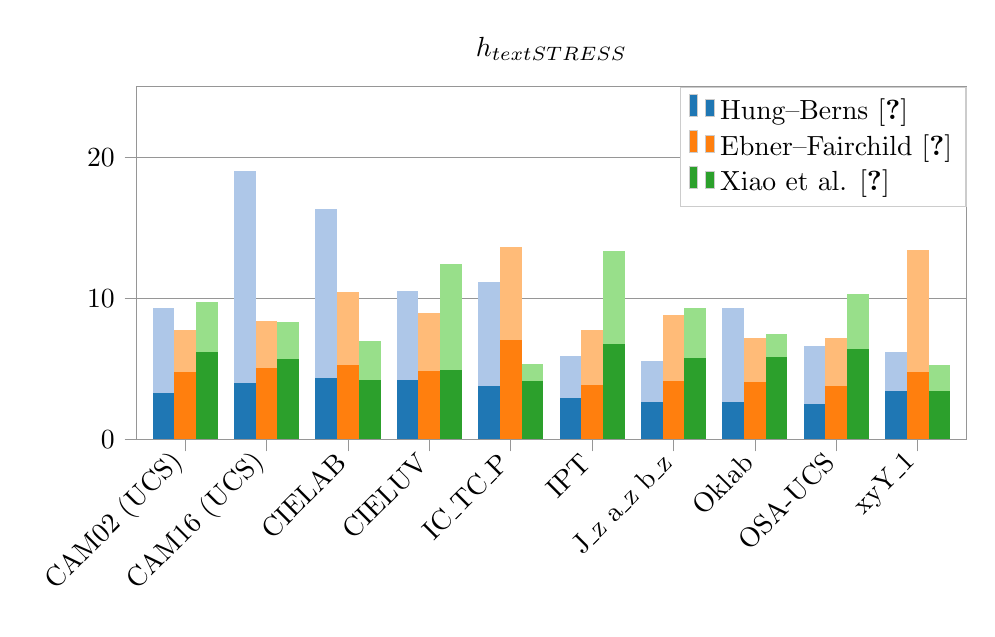
\begin{tikzpicture}

\definecolor{color0}{rgb}{0.12156862745098,0.466666666666667,0.705882352941177}
\definecolor{color1}{rgb}{0.682352941176471,0.780392156862745,0.909803921568627}
\definecolor{color2}{rgb}{1,0.498039215686275,0.0549019607843137}
\definecolor{color3}{rgb}{1,0.733333333333333,0.470588235294118}
\definecolor{color4}{rgb}{0.172549019607843,0.627450980392157,0.172549019607843}
\definecolor{color5}{rgb}{0.596078431372549,0.874509803921569,0.541176470588235}

\begin{axis}[
axis line style={white!58.8235294117647!black},
height=0.5\textwidth,
legend cell align={left},
legend style={fill opacity=1, draw opacity=1, text opacity=1, at={(1,1)}, draw=white!80!black},
tick align=outside,
tick pos=left,
title={\(\displaystyle h_{text{STRESS}}\)},
width=\textwidth,
x grid style={white!58.8235294117647!black},
xmin=-0.6, xmax=9.6,
xtick style={color=white!58.8235294117647!black},
xtick={0,1,2,3,4,5,6,7,8,9},
xticklabel style={rotate=45.0,anchor=east},
xticklabels={
  CAM02 (UCS),
  CAM16 (UCS),
  CIELAB,
  CIELUV,
  IC\_TC\_P,
  IPT,
  J\_z a\_z b\_z,
  Oklab,
  OSA-UCS,
  xyY\_1
},
y grid style={white!58.8235294117647!black},
ymajorgrids,
ymin=0, ymax=25,
ytick style={color=white!58.8235294117647!black},
yticklabel style={anchor=east}
]
\draw[draw=none,fill=color0] (axis cs:-0.4,0) rectangle (axis cs:-0.133333333333333,3.26752096358107);
\addlegendimage{ybar,ybar legend,draw=none,fill=color0}
\addlegendentry{Hung--Berns \cite{hung}}

\draw[draw=none,fill=color0] (axis cs:0.6,0) rectangle (axis cs:0.866666666666667,4.03663610711868);
\draw[draw=none,fill=color0] (axis cs:1.6,0) rectangle (axis cs:1.86666666666667,4.34856818798823);
\draw[draw=none,fill=color0] (axis cs:2.6,0) rectangle (axis cs:2.86666666666667,4.21626028738579);
\draw[draw=none,fill=color0] (axis cs:3.6,0) rectangle (axis cs:3.86666666666667,3.7957739893557);
\draw[draw=none,fill=color0] (axis cs:4.6,0) rectangle (axis cs:4.86666666666667,2.92119683105356);
\draw[draw=none,fill=color0] (axis cs:5.6,0) rectangle (axis cs:5.86666666666667,2.68536426894407);
\draw[draw=none,fill=color0] (axis cs:6.6,0) rectangle (axis cs:6.86666666666667,2.63371950519244);
\draw[draw=none,fill=color0] (axis cs:7.6,0) rectangle (axis cs:7.86666666666667,2.49530998013144);
\draw[draw=none,fill=color0] (axis cs:8.6,0) rectangle (axis cs:8.86666666666667,3.44018748653443);
\draw[draw=none,fill=color1] (axis cs:-0.4,3.26752096358107) rectangle (axis cs:-0.133333333333333,9.31831019858184);
\draw[draw=none,fill=color1] (axis cs:0.6,4.03663610711868) rectangle (axis cs:0.866666666666667,19.0454890766849);
\draw[draw=none,fill=color1] (axis cs:1.6,4.34856818798823) rectangle (axis cs:1.86666666666667,16.3352901071817);
\draw[draw=none,fill=color1] (axis cs:2.6,4.21626028738579) rectangle (axis cs:2.86666666666667,10.5220652280729);
\draw[draw=none,fill=color1] (axis cs:3.6,3.7957739893557) rectangle (axis cs:3.86666666666667,11.1890830346539);
\draw[draw=none,fill=color1] (axis cs:4.6,2.92119683105356) rectangle (axis cs:4.86666666666667,5.89478443004315);
\draw[draw=none,fill=color1] (axis cs:5.6,2.68536426894407) rectangle (axis cs:5.86666666666667,5.55970441646704);
\draw[draw=none,fill=color1] (axis cs:6.6,2.63371950519244) rectangle (axis cs:6.86666666666667,9.31997777958706);
\draw[draw=none,fill=color1] (axis cs:7.6,2.49530998013144) rectangle (axis cs:7.86666666666667,6.59231944961339);
\draw[draw=none,fill=color1] (axis cs:8.6,3.44018748653443) rectangle (axis cs:8.86666666666667,6.18717018996993);
\draw[draw=none,fill=color2] (axis cs:-0.133333333333333,0) rectangle (axis cs:0.133333333333333,4.75235322590395);
\addlegendimage{ybar,ybar legend,draw=none,fill=color2}
\addlegendentry{Ebner--Fairchild \cite{ebner}}

\draw[draw=none,fill=color2] (axis cs:0.866666666666667,0) rectangle (axis cs:1.13333333333333,5.07600805665883);
\draw[draw=none,fill=color2] (axis cs:1.86666666666667,0) rectangle (axis cs:2.13333333333333,5.30715095336481);
\draw[draw=none,fill=color2] (axis cs:2.86666666666667,0) rectangle (axis cs:3.13333333333333,4.82895376092783);
\draw[draw=none,fill=color2] (axis cs:3.86666666666667,0) rectangle (axis cs:4.13333333333333,7.04859738515855);
\draw[draw=none,fill=color2] (axis cs:4.86666666666667,0) rectangle (axis cs:5.13333333333333,3.8585452834895);
\draw[draw=none,fill=color2] (axis cs:5.86666666666667,0) rectangle (axis cs:6.13333333333333,4.11463844121543);
\draw[draw=none,fill=color2] (axis cs:6.86666666666667,0) rectangle (axis cs:7.13333333333333,4.05730886560147);
\draw[draw=none,fill=color2] (axis cs:7.86666666666667,0) rectangle (axis cs:8.13333333333333,3.81297237590754);
\draw[draw=none,fill=color2] (axis cs:8.86666666666667,0) rectangle (axis cs:9.13333333333333,4.75045818919244);
\draw[draw=none,fill=color3] (axis cs:-0.133333333333333,4.75235322590395) rectangle (axis cs:0.133333333333333,7.75477854637728);
\draw[draw=none,fill=color3] (axis cs:0.866666666666667,5.07600805665883) rectangle (axis cs:1.13333333333333,8.3610550997474);
\draw[draw=none,fill=color3] (axis cs:1.86666666666667,5.30715095336481) rectangle (axis cs:2.13333333333333,10.4461969203768);
\draw[draw=none,fill=color3] (axis cs:2.86666666666667,4.82895376092783) rectangle (axis cs:3.13333333333333,8.96951788031229);
\draw[draw=none,fill=color3] (axis cs:3.86666666666667,7.04859738515855) rectangle (axis cs:4.13333333333333,13.6280487760657);
\draw[draw=none,fill=color3] (axis cs:4.86666666666667,3.8585452834895) rectangle (axis cs:5.13333333333333,7.72233957150083);
\draw[draw=none,fill=color3] (axis cs:5.86666666666667,4.11463844121543) rectangle (axis cs:6.13333333333333,8.80555808428739);
\draw[draw=none,fill=color3] (axis cs:6.86666666666667,4.05730886560147) rectangle (axis cs:7.13333333333333,7.16171792324175);
\draw[draw=none,fill=color3] (axis cs:7.86666666666667,3.81297237590754) rectangle (axis cs:8.13333333333333,7.17861133082468);
\draw[draw=none,fill=color3] (axis cs:8.86666666666667,4.75045818919244) rectangle (axis cs:9.13333333333333,13.4354916910975);
\draw[draw=none,fill=color4] (axis cs:0.133333333333333,0) rectangle (axis cs:0.4,6.20819583068422);
\addlegendimage{ybar,ybar legend,draw=none,fill=color4}
\addlegendentry{Xiao et al. \cite{xiao}}

\draw[draw=none,fill=color4] (axis cs:1.13333333333333,0) rectangle (axis cs:1.4,5.72257615772014);
\draw[draw=none,fill=color4] (axis cs:2.13333333333333,0) rectangle (axis cs:2.4,4.23955931207377);
\draw[draw=none,fill=color4] (axis cs:3.13333333333333,0) rectangle (axis cs:3.4,4.94778942179497);
\draw[draw=none,fill=color4] (axis cs:4.13333333333333,0) rectangle (axis cs:4.4,4.16705224310084);
\draw[draw=none,fill=color4] (axis cs:5.13333333333333,0) rectangle (axis cs:5.4,6.77347388639466);
\draw[draw=none,fill=color4] (axis cs:6.13333333333333,0) rectangle (axis cs:6.4,5.79350009458331);
\draw[draw=none,fill=color4] (axis cs:7.13333333333333,0) rectangle (axis cs:7.4,5.83206308550634);
\draw[draw=none,fill=color4] (axis cs:8.13333333333333,0) rectangle (axis cs:8.4,6.37866193244546);
\draw[draw=none,fill=color4] (axis cs:9.13333333333333,0) rectangle (axis cs:9.4,3.40752186432332);
\draw[draw=none,fill=color5] (axis cs:0.133333333333333,6.20819583068422) rectangle (axis cs:0.4,9.7428242142996);
\draw[draw=none,fill=color5] (axis cs:1.13333333333333,5.72257615772014) rectangle (axis cs:1.4,8.3428798127558);
\draw[draw=none,fill=color5] (axis cs:2.13333333333333,4.23955931207377) rectangle (axis cs:2.4,6.98657068830182);
\draw[draw=none,fill=color5] (axis cs:3.13333333333333,4.94778942179497) rectangle (axis cs:3.4,12.4312850951466);
\draw[draw=none,fill=color5] (axis cs:4.13333333333333,4.16705224310084) rectangle (axis cs:4.4,5.35549940442929);
\draw[draw=none,fill=color5] (axis cs:5.13333333333333,6.77347388639466) rectangle (axis cs:5.4,13.3872434394625);
\draw[draw=none,fill=color5] (axis cs:6.13333333333333,5.79350009458331) rectangle (axis cs:6.4,9.2918389298864);
\draw[draw=none,fill=color5] (axis cs:7.13333333333333,5.83206308550634) rectangle (axis cs:7.4,7.46796819499847);
\draw[draw=none,fill=color5] (axis cs:8.13333333333333,6.37866193244546) rectangle (axis cs:8.4,10.314700143108);
\draw[draw=none,fill=color5] (axis cs:9.13333333333333,3.40752186432332) rectangle (axis cs:9.4,5.26331086619812);
\end{axis}

\end{tikzpicture}
